\section{连续分布、密度与分位数}
\label{sec:05-Probability/03-Random-Variables/03}

值班群里贴出来的接口监控只有三个数：p50 是 42 毫秒，p99 是 380 毫秒，最大 2.1 秒。没人问``响应时间恰好等于 100 毫秒的概率是多少''，服务等级协议里也不会这么写。

上一节那张表在这里造不出来。响应时间可以是 42.0 毫秒，也可以是 42.000317 毫秒，取值填满一整段区间。若照 PMF 的办法给每个实数点分一份质量，两条路都是死路：每点分正数，不可数个正数加起来必然发散；每点分零，可数可加性又拼不回总量 1。可数求和这件工具在不可数集合上失效，得换一件。

\subsection{把质量摊成浓度}

先退回一个算得动的问题。设下一班车到站的时刻在 \([0,10]\) 分钟上均匀分布，落在 \([2,5]\) 的概率就是 \(3/10\)——概率与区间长度成正比，比例系数 \(1/10\)。这个系数说的是每单位时间承载多少概率，叫它密度。

一般情形照这条思路写下来。

\begin{definition}
若存在非负函数 \(f_X\)，使得对任意 \(a<b\) 有
\[
P(a<X\le b)=\int_a^b f_X(x)\,dx,
\]
则称 \(X\) 为连续随机变量，\(f_X\) 为它的概率密度函数（PDF）。令 \(a\to-\infty\)、\(b\to+\infty\) 即得归一化条件 \(\int_{-\infty}^{\infty}f_X(x)\,dx=1\)。
\end{definition}

积分号一进来，单点概率就塌了：\(P(X=x)=\int_x^x f_X(t)\,dt=0\)。于是区间的开闭不再影响结果，\(P(a<X<b)\) 与 \(P(a\le X\le b)\) 一样大。上一节离散情形里那种要不要把端点补回来的小心翼翼，这里全免了。

换来一条容易读错的结论：概率为零不等于不可能。车总会在某个时刻到，而那个时刻属于一个概率为零的单点集。可数可加性只承诺可数个互斥事件的概率能相加，\([0,10]\) 里的点有不可数个，把它们的零概率``加起来''这个动作压根没有定义，也就谈不上矛盾。这条界限要说清楚需要测度论的语言，交代在\hyperref[ch:101]{``测度、积分与条件期望：为现代概率回填地基''}。

\subsection{密度值可以大于 1}

从离散过渡过来，这是最容易翻的一条船。PMF 的值 \(p_X(x)=P(X=x)\) 本身是某个事件的概率，永远不超过 1。密度不是任何事件的概率，它没有这条上界。

取 \(X\sim\Uniform(0,0.5)\)。取值全挤在长度 \(0.5\) 的区间里，总量 1 只能靠把密度抬到 \(f_X(x)=2\) 才凑得出来。

\begin{center}
\begin{tikzpicture}[x=1.5cm,y=1.05cm,font=\footnotesize,>=stealth]
  \begin{scope}
    \draw[dashed,black!35] (0,1) -- (2.6,1);
    \fill[blue!16] (0,0) rectangle (2,0.5);
    \draw[blue!65!black,thick] (0,0) -- (0,0.5) -- (2,0.5) -- (2,0);
    \draw[->] (-0.15,0) -- (2.8,0) node[right] {\(x\)};
    \draw[->] (0,-0.14) -- (0,2.55);
    \node[below] at (2,-0.08) {\(2\)};
    \node[left,black!60] at (-0.05,1) {\(1\)};
    \node[left,black!60] at (-0.05,0.5) {\(0.5\)};
    \node[above,black!70] at (1.0,0.55) {面积 \(=1\)};
    \node at (1.0,2.15) {\(\Uniform(0,2)\)};
  \end{scope}
  \begin{scope}[xshift=4.9cm]
    \draw[dashed,black!35] (0,1) -- (2.6,1);
    \fill[orange!25] (0,0) rectangle (0.5,2);
    \draw[orange!75!black,thick] (0,0) -- (0,2) -- (0.5,2) -- (0.5,0);
    \draw[->] (-0.15,0) -- (2.8,0) node[right] {\(x\)};
    \draw[->] (0,-0.14) -- (0,2.55);
    \node[below] at (0.5,-0.08) {\(0.5\)};
    \node[left,black!60] at (-0.05,1) {\(1\)};
    \node[left,black!60] at (-0.05,2) {\(2\)};
    \node[right,black!70] at (0.6,1.4) {面积 \(=1\)};
    \node at (1.5,2.15) {\(\Uniform(0,0.5)\)};
  \end{scope}
\end{tikzpicture}

\emph{两块图形围出的面积都是 1，横向压缩多少倍，纵向就得抬高多少倍。虚线是高度 1 的参考线：右边那条密度取值 2，越过了它，却没有违反任何一条概率公理——密度不是概率，概率是密度乘长度。}
\end{center}

人口密度是同一个比方：每平方公里多少人，乘上面积才是人数。密度还有一个附带的后果，它带单位。把响应时间的记录从毫秒换成秒，同一个分布的密度值会整体乘以 1000，而任何一个区间的概率纹丝不动。一个带单位的量当然可以大于 1，这跟温度可以超过 100 是一回事。

做模型的人早晚会撞上这件事。连续变量的似然值大于 1、对数似然算出来是正数，都是合法结果，不是代码写错了——似然是密度值，不是概率。

\subsection{分布函数才是通用的那一个}

密度只对连续变量有定义，PMF 只对离散变量有定义。横跨两边的是分布函数，它的定义从上一节起就没有变过：
\[
F_X(x)=P(X\le x).
\]
有密度时，\(F_X(x)=\int_{-\infty}^{x}f_X(t)\,dt\)；在 \(F_X\) 可导的点上反过来有 \(f_X(x)=F_X'(x)\)。累计存量与瞬时速率的那套关系，在这里原样复用。

拿一个能算完的例子摆着：\(f_X(x)=2x\)（\(0\le x\le1\)），积分得 \(F_X(x)=x^2\)。密度向右递增，CDF 就在右侧爬得陡。

\begin{center}
\begin{tikzpicture}[x=2.8cm,y=2cm,>=stealth,every node/.style={font=\small}]
  \begin{scope}[xshift=-2.2cm]
    \draw[->] (-0.08,0) -- (1.15,0) node[right] {\(x\)};
    \draw[->] (0,-0.05) -- (0,2.2) node[above left] {\(f_X(x)\)};
    \draw[blue!70!black,thick] (0,0) -- (1,2);
    \fill[blue!20] (0.5,0) -- (0.5,1) -- (0.75,1.5) -- (0.75,0) -- cycle;
    \draw[dashed] (0.5,0) -- (0.5,1);
    \draw[dashed] (0.75,0) -- (0.75,1.5);
    \node[font=\footnotesize] at (0.63,0.35) {面积};
    \node at (0.5,-0.25) {\(a\)};
    \node at (0.75,-0.25) {\(b\)};
    \node at (0.5,2.35) {PDF：局部浓度};
  \end{scope}
  \begin{scope}[xshift=2.0cm]
    \draw[->] (-0.08,0) -- (1.15,0) node[right] {\(x\)};
    \draw[->] (0,-0.05) -- (0,1.2) node[above left] {\(F_X(x)\)};
    \draw[blue!70!black,thick] plot[domain=0:1,samples=50] (\x,{\x*\x});
    \draw[dashed] (0.5,0) -- (0.5,0.25) -- (0,0.25);
    \draw[dashed] (0.75,0) -- (0.75,0.5625) -- (0,0.5625);
    \draw[<->,gray!80] (0.82,0.25) -- (0.82,0.5625)
      node[midway,right] {区间概率};
    \node at (0.5,1.35) {CDF：累计存量};
  \end{scope}
\end{tikzpicture}

\emph{左图曲线下 \([a,b]\) 的面积，等于右图累计概率从 \(F(a)\) 到 \(F(b)\) 的增量。}
\end{center}

图里那句``面积才是概率''值得多停一秒。要算 \(P(1/2<X\le 3/4)\)，答案是 \(F_X(3/4)-F_X(1/2)=5/16\)，不是纵坐标 \(f_X(1/2)=1\) 或 \(f_X(3/4)=1.5\)。密度曲线的高度只在乘上宽度之后才有概率的含义。

\(F\) 的通用性在混合分布上兑现得最明显。保险理赔的数据里大量保单赔付为零，其余在正实数上连续分布；测量仪器有检测下限，低于下限的读数一律归并成同一个值。这两种数据里，PMF 只抓得住点质量，PDF 只描述得了连续段，谁都拼不出完整的分布。以 \(1/2\) 概率取 0、以 \(1/2\) 概率在 \([0,1]\) 上均匀，写成分布函数就是
\[
F_X(x)=
\begin{cases}
0,&x<0,\\
\tfrac12+\tfrac12 x,&0\le x\le1,\\
1,&x>1,
\end{cases}
\]
在 \(x=0\) 处竖直跳 \(1/2\)（那是点质量），之后以斜率 \(1/2\) 爬到 1（那是连续部分）。竖直的跳跃和倾斜的上升写在同一条曲线上，各占多少权重一望即知。

\begin{proposition}
任一随机变量的 \(F_X\) 单调不减、右连续，且 \(\lim_{x\to-\infty}F_X(x)=0\)、\(\lim_{x\to+\infty}F_X(x)=1\)。反过来，满足这四条的函数必是某个随机变量的分布函数。
\end{proposition}

正向逐条对账即可：单调来自事件包含 \(\set{X\le x}\subseteq\set{X\le x'}\)；右连续来自 \(x_n\downarrow x\) 时 \(\set{X\le x_n}\) 的交恰为 \(\set{X\le x}\)，再用概率的连续性；两端极限同理，把事件列取到空集和全空间。反向的构造更有意思，它要用到本节剩下的那个工具，稍后就会看到。

\subsection{把问题倒过来问}

CDF 问的是``走到 \(x\)，左边攒了多少概率''；实践中更常出现的是反方向：``要攒够 \(p\)，得走到哪里''。

\begin{definition}
\(X\) 的分位数函数为
\[
Q(p)=\inf\set{x\in\R\given F_X(x)\ge p},\qquad 0<p<1.
\]
\end{definition}

为什么用下确界，不直接写反函数？两种情形会让反函数失效。\(F\) 有跳跃时（离散或混合分布），跳跃跨过的那些 \(p\) 值根本没有 \(x\) 与之对应；\(F\) 有水平段时（那一段区间的概率为零），同一个 \(p\) 对应一整段 \(x\)。下确界在前一种情形里选中跳跃的落点，在后一种情形里选中水平段的左端。\(F\) 连续且严格递增时它退化成普通反函数，两个记号 \(Q\) 与 \(F^{-1}\) 在文献里混着用。

\begin{center}
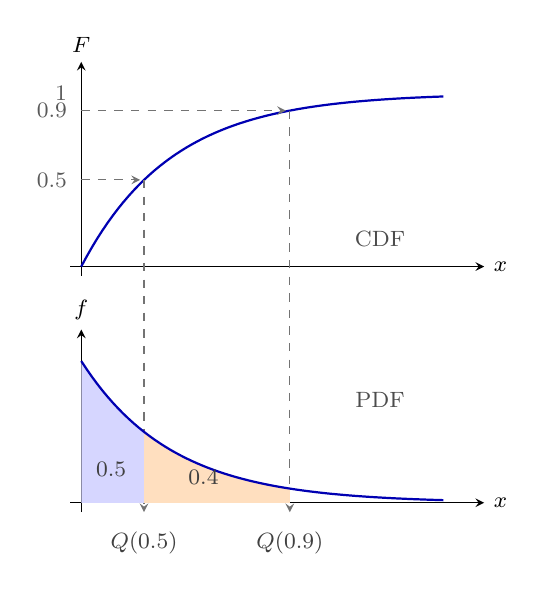
\begin{tikzpicture}[x=1.15cm,y=1cm,font=\footnotesize,>=stealth]
  \draw[->] (-0.12,3.0) -- (4.45,3.0) node[right] {\(x\)};
  \draw[->] (0,2.88) -- (0,5.6) node[above] {\(F\)};
  \draw[blue!70!black,thick] plot[domain=0:4,samples=70] (\x,{3.0+2.2*(1-exp(-\x))});
  \draw[dashed,->,black!55] (0,4.1) -- (0.65,4.1);
  \draw[dashed,->,black!55] (0,4.98) -- (2.26,4.98);
  \node[left,black!65] at (-0.05,4.1) {\(0.5\)};
  \node[left,black!65] at (-0.05,4.98) {\(0.9\)};
  \node[left,black!65] at (-0.05,5.2) {\(1\)};
  \node[black!70] at (3.3,3.35) {CDF};
  \draw[dashed,->,black!55] (0.693,4.1) -- (0.693,-0.12);
  \draw[dashed,->,black!55] (2.303,4.98) -- (2.303,-0.12);
  \draw[->] (-0.12,0) -- (4.45,0) node[right] {\(x\)};
  \draw[->] (0,-0.12) -- (0,2.2) node[above] {\(f\)};
  \fill[blue!16] (0,0) -- plot[domain=0:0.693,samples=25] (\x,{1.8*exp(-\x)}) -- (0.693,0) -- cycle;
  \fill[orange!25] (0.693,0) -- plot[domain=0.693:2.303,samples=25] (\x,{1.8*exp(-\x)}) -- (2.303,0) -- cycle;
  \draw[blue!70!black,thick] plot[domain=0:4,samples=70] (\x,{1.8*exp(-\x)});
  \node[black!75] at (0.33,0.42) {\(0.5\)};
  \node[black!75] at (1.35,0.32) {\(0.4\)};
  \node[below,black!75] at (0.693,-0.24) {\(Q(0.5)\)};
  \node[below,black!75] at (2.303,-0.24) {\(Q(0.9)\)};
  \node[black!70] at (3.3,1.3) {PDF};
\end{tikzpicture}

\emph{上下两幅共用一条横轴，画的是 \(F(x)=1-e^{-x}\)。求分位数的动作是：在上图纵轴找到 \(p\)，横着走到曲线，再垂直落到横轴。落点把下图的密度切开，左侧那块面积正好是 \(p\)。概率从 \(0.5\) 加到 \(0.9\) 只多了 \(0.4\)，位置却从 \(0.69\) 推到 \(2.30\)——尾部的分位数走得远，是因为 \(F\) 在那里已经接近水平。}
\end{center}

这张图也解释了分位数为什么在实际工作里比密度出现得更频繁。尾部风险的度量 VaR 就是损失分布的 \(0.95\) 或 \(0.99\) 分位数；模型校准检查的是``声称的 \(90\%\) 预测区间是否真的盖住了 \(90\%\) 的实测值''（见\hyperref[ch:092]{``统计决策与可信预测：模型给出概率之后怎样行动''}），比对的两端都是分位数；分位数回归干脆不建模条件均值，直接把若干条条件分位数当作输出。这几件事有一个共同点：它们要的答案就写在 \(F^{-1}\) 上，中途不必经过密度。密度得先估出一条曲线、再积分才能回答概率问题，而样本分位数把数据排序之后几乎可以直接读。

稳健性是另一层理由。往 100 个收入数据里塞进一位亿万富翁，均值立刻被拉走，中位数几乎不动——收入统计通常汇报中位数，原因就在这里。分位数与均值的落差还能读出分布的偏斜：\(\Exp(1)\) 的中位数解 \(1-e^{-m}=1/2\) 得 \(m=\ln 2\approx0.693\)，明显小于均值 1，少数很长的等待把均值抬了上去，中位数不受影响。均值大于中位数是右偏的标志，反过来是左偏。

\begin{remark}
两条边界值得记一下。离散分布的中位数可能不唯一——概率质量恰好把 \(0.5\) 夹在中间时，一整段区间都符合定义，这是广义逆从跳跃处继承来的正常现象。另一条是工程上的：各家软件对样本分位数的插值约定不同，同一批数据算出的 p99 可以差一点点。那是有限样本下加权方式的实现选择，不是理论含糊。
\end{remark}

回到刚才欠下的那笔账。给一个满足四条性质的 \(F\)，取 \(U\sim\Uniform(0,1)\) 并令 \(X=Q(U)\)，就有 \(P(X\le x)=P(U\le F(x))=F(x)\)，构造完成。这句话的分量远超一个存在性证明——它是几乎所有采样器的底层机制，下一节会把它拆开讲。

\subsection{读密度表达式，先问它在哪儿生效}

密度公式脱离定义域就不成立。指数分布的密度写作 \(\lambda e^{-\lambda x}\) 时必须附带 \(x\ge0\)；忘了在负半轴上补零而直接在整条实轴上积分，会得到一个发散的结果。看到密度表达式，第一件事是问它在哪些 \(x\) 上非零。

支撑集是另一处容易含糊的地方。它指的是那些``任意小的邻域都有正概率''的点构成的闭集，判断依据是邻域而不是该点的密度值。\(f_X(x)=2x\) 在 \(x=0\) 处密度为零，可 \(P(0\le X<\varepsilon)=\varepsilon^2>0\) 对每个 \(\varepsilon>0\) 都成立，所以 0 照样在支撑集里。

分位数函数已经把``给概率求位置''这条路打通了。下一节反着用它：喂一个均匀随机数进去，出来的是服从目标分布的样本。这不是一个孤立的技巧——它是随机变量变换的一个特例，而变换公式里那个导数因子，正是密度在拉伸和压缩下的换算方式。
